%%
%% Author: dariochinelli
%% 2021-01-25
%%

\section{Condensazione di Bose-Einstein}

Consideriamo bosoni con spin $= 0$ e massa $m \not = 0$ non interagenti.
Tutte le particelle tendono ad andare nel livello $E_s=0$.
\begin{equation}
\begin{split}
\frac{ n_s}{g_s } & = \frac{ 1}{e^{ \alpha + \beta E_s } - 1 } \\
\Rightarrow \frac{ n_0}{g_0 } & = \frac{ 1}{e^{ \alpha + \beta E_0 } - 1 } = \frac{ n_0}{g_0 } = \frac{ 1}{e^{ \alpha } - 1 } \\
\Rightarrow N & = \frac{ 1}{e^{ \alpha } - 1 }
\end{split}
\end{equation}

Notare che $g_0 = 1$ poiché $g(E) \sim E^{ \frac{ 1}{2 }}$ ma poiché $g(0)=0$ non ha senso fisico si assume che il minimo valore di $g$ sia 1.

Dato che $N$ (numero di particelle) è grande, allora, essendo $e^{ \alpha } = 1 + \frac{ 1}{N }\simeq 1 \Rightarrow \alpha \sim 0$ allora:
$$ N \simeq \frac{ 1}{1 + \alpha - 1 } \Rightarrow \alpha \simeq \frac{ 1}{N }$$
Il numero totale di particelle è dato da $N = \sum_s n_s = n_0 + n_e = n_0 + \int_0^{\infty} n(E)dE$ dove $n_0$ è il numero di particelle nello stato fondamentale e $n_e$ il numero di particelle negli stati eccitati.
Poiché però:
\begin{equation}
n(E)dE = \frac{ g(E)dE}{e^{ \alpha + \beta E_s } - 1 } \quad \mbox{ e } \quad g(E) dE= \frac{ 4 \pi V (2m^3)^\frac{ 1}{2 } E^\frac{ 1}{2 } }{ h^3} dE
\end{equation}

\begin{equation}
\begin{split}
N & = n_0 + C \int_0^{\infty} \frac{ E^{ \frac{ 1}{2 } }}{e^{\alpha + \beta E } -1 }dE = n_0 + C (kT)^{ \frac{ 3}{2 } } \int_0^{\infty} \frac{ z^{\frac{ 1}{2 } dz}}{e^{z+\alpha } - 1} \quad
\mbox{dove} \quad
\begin{cases}
	z = \beta E \\
	dE = k T dZ
\end{cases}
\end{split}
\end{equation}
Questo integrale, che chiameremo $G(\alpha)$, è estremamente complicato, ma si ha che:
\begin{equation}
\begin{cases}
	\alpha \mbox{ grande} \quad G(\alpha) = \frac{ \sqrt{\pi}}{2 } e^{ - \alpha } \\
	\alpha \mbox{ piccolo} \quad G(0) = 2.612 \sqrt{\frac{ \pi}{4 }}
\end{cases}
\end{equation}
Nel nostro caso $\alpha$ è piccolo essendo $N$ grande, e dunque si può approssimare scrivendo che 
\begin{equation}
\begin{split}
	n_0 & = N - C (kT)^{ \frac{ 3}{2 } } \sqrt{\frac{ \pi}{4 }} 2.612 = N \Bigl[ 1 - \frac{ T}{T_c } \Bigr] \\
	\mbox{dove } T_c & = (CN)^{ \frac{ 3}{2 } }  = C \Bigl(  \frac{ N}{V }  \Bigr)^{ \frac{ 3}{2 } } \sim e^{ \frac{ 3}{2 } } 
\end{split}
\end{equation}
per cui $T_c$ è una \underline{temperatura critica} che va come la densità alla $\frac{ 2}{3 }$.

	\newpage

\begin{figure}[h]
\centering
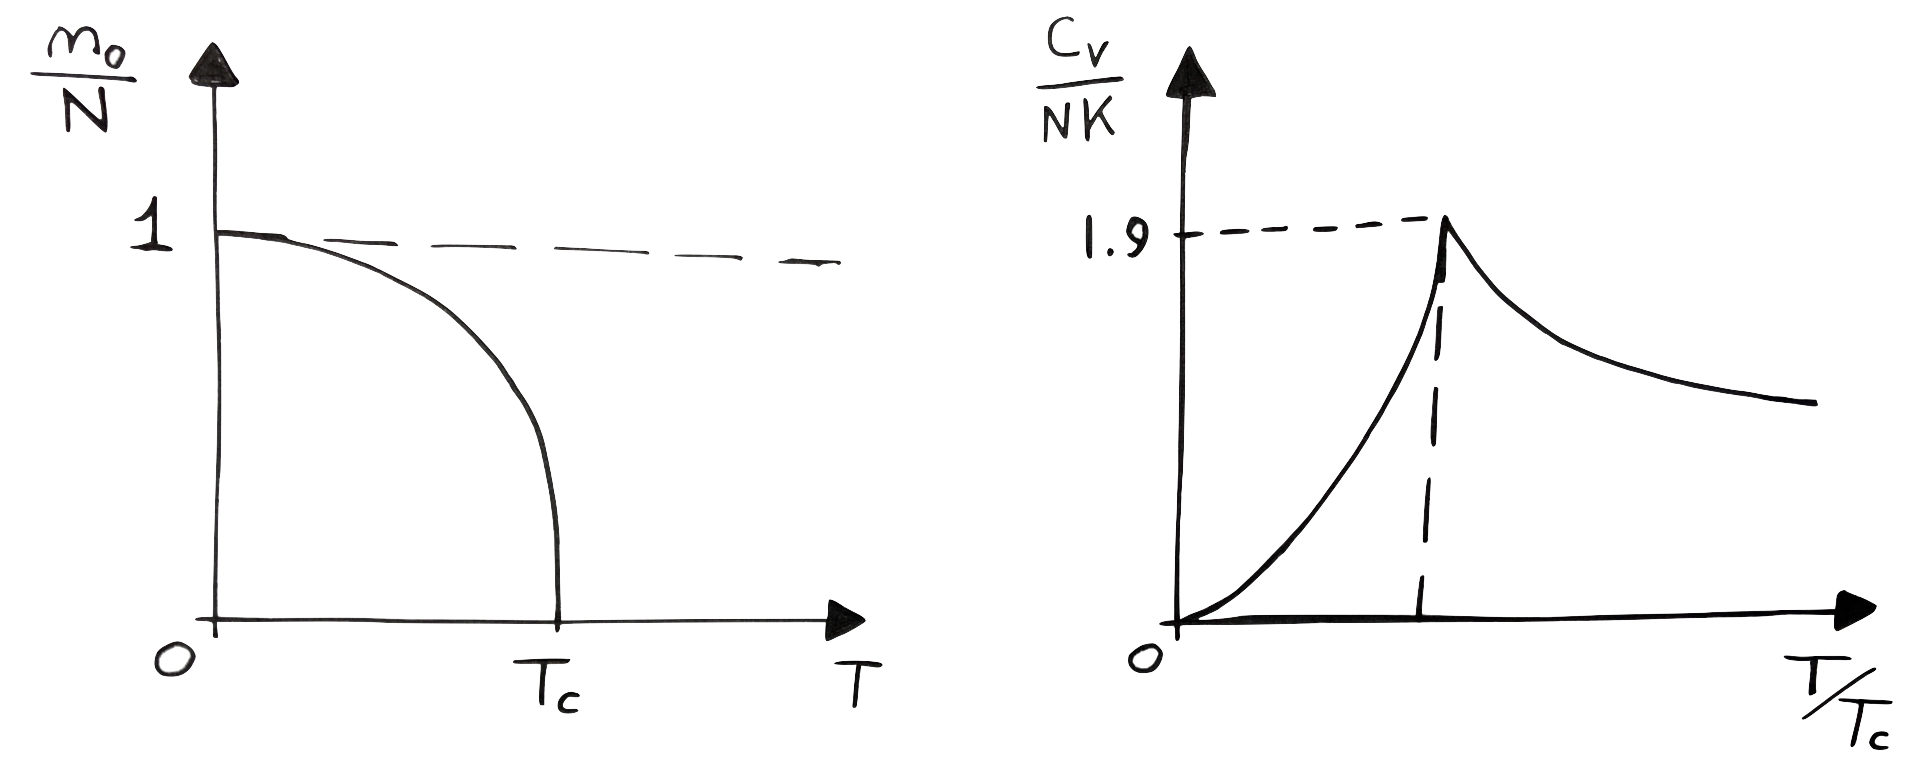
\includegraphics[scale=0.25]{/andamenti_Cv_T}
\end{figure}
Il numero di particelle nello stato fondamentale rimane grande fino a che $T < T_c$.
Al di sotto della temperatura critica le particelle sono condensate nel livello energetico minore di energia, cioè si ha il fenomeno della \underline{condensazione di Bose-Einstein}.
\begin{equation}
C_V = N K \Bigl(  \frac{ T}{T_c }  \Bigr) C \quad \mbox{dove} \quad C \to 1.9
\end{equation} 

Un fenomeno affascinante, affine alla condensazione di Bose-Einstein, è la superconduttività dell'elio liquido, per cui si consiglia di leggere il seguente paragrafo:

\textit{"Bose Condensation and liquid helium", pag 399-404, da Eisnerg-Resnick, Quantum Physics of atoms, molecules, solids, nuclei and particles}.


